%% \documentclass[compress,12pt]{beamer}

%% \usepackage{mathrsfs}
%% \usepackage{stmaryrd} % \llbracket

%% \newcommand{\bv}[1]{{\boldsymbol{#1}}}

%% % This puts serifs on equations, which is not standard in Beamer talks.
%% % \usefonttheme[onlymath]{serif}

%% \usetheme{Darmstadt} % Berlin with no bottom nav and rounded blocks, pretty nice, a bit too much at top though
%% \usecolortheme{sidebartab}

%% \usepackage{times}
%% \usepackage{units}

%% \setbeamercovered{invisible}
%% \logo{\includegraphics[width=.5in]{figures/word3}}

%% \title{Using LibMesh for Scientific Computations}
%% \subtitle{\url{https://github.com/libMesh/libmesh}}
%% \author{Roy Stogner \and John Peterson}
%% \date{November 3, 2005}
%% \institute{EM 397.4 -- Grid Generation \& Adaptive Grids}

%% \begin{document}

%% \begin{frame}
%%   \titlepage
%% \end{frame}



%% %%%%%%%%%%%%%%%%%%%%%%%%%%%%%%%%%%%%%%%%%%%%%%%%%%%%%%%%%%%%%%%%%%%%%%%%%%%%%%%
%% \begin{frame}{Outline}
%%   \begin{itemize}
%%     \item A Model Problem
%%     \item Galerkin FE Method
%%     \item Penalty Boundary Conditions
%%     \item Adaptivity
%%     \item Error Indicators
%%     \item 1D Example
%%   \end{itemize}
%% \end{frame}

\section{Adaptive Mesh Refinement}

\subsection{Model Problem}


%%%%%%%%%%%%%%%%%%%%%%%%%%%%%%%%%%%%%%%%%%%%%%%%%%%%%%%%%%%%%%%%%%%%%%%%%%%%%%%
\begin{frame}{Model Problem}
\begin{itemize}
  \item Consider the 1D model ODE
    \begin{equation}
      \left\{
	\begin{array}{ccc}
	  -u'' + bu' +cu &=& f \hspace{.25in} \in \hspace{.1in} \Omega = (0,L) \\
	  u(0) =  u_0   && \\
	  u(L) =  u_L	&&
	\end{array}
	\right.
    \end{equation}

  \item with weak form
    \begin{equation}
      \int_{\Omega} \left( u' v' + b u' v + cuv \right) \; dx = \int_{\Omega} fv \; dx
    \end{equation}

    for every $v \in H^1_0 (\Omega)$.
\end{itemize}
\end{frame}


%%%%%%%%%%%%%%%%%%%%%%%%%%%%%%%%%%%%%%%%%%%%%%%%%%%%%%%%%%%%%%%%%%%%%%%%%%%%%%%
\begin{frame}{Model Problem (cont.)}
\begin{itemize}
\item The analogous $d$-dimensional problem with $\Omega \subset \mathbb{R}^d$
  and boundary $\partial \Omega$ is
    \begin{equation}
      \left\{
	\begin{array}{ccl}
	  -\Delta u + \bv{b} \cdot \nabla u + cu &=& f
	  \hspace{.25in} \in \hspace{.1in} \Omega  \\
	  \phantom{-\Delta u + \bv{b} \cdot \nabla u + c}u & = & g
	  \hspace{.25in} \in \hspace{.1in} \partial \Omega
	\end{array}
	\right.
    \end{equation}

  \item with weak form
    \begin{equation}
      \int_{\Omega} \left( \nabla u \cdot \nabla v + (\bv{b} \cdot \nabla u) v + cuv \right) \; dx = \int_{\Omega} fv \; dx
    \end{equation}

\end{itemize}

\end{frame}


%%%%%%%%%%%%%%%%%%%%%%%%%%%%%%%%%%%%%%%%%%%%%%%%%%%%%%%%%%%%%%%%%%%%%%%%%%%%%%%
\begin{frame}{Model Problem (cont.)}
\begin{itemize}
\item The finite element method works with the weak form, replacing the trial and
  test functions $u,v$ with their approximations $u^h, v^h$, and summing the
  contributions of the element integrals
  \gdef\eqneltint{      \sum_{e=1}^{N_e} \int_{\Omega_e}
      \left( \nabla u^h \cdot \nabla v^h + (\bv{b} \cdot \nabla u^h) v^h + cu^h v^h
      -fv^h \right)\;  dx=0}
    \begin{equation}\label{eqn:element_integrals}
      \eqneltint
    \end{equation}

  \item Remark: We considered here a standard piecewise continuous finite element basis.
    In general, $\nabla u^h$ will have a jump discontinuity across element boundaries.
\end{itemize}
\end{frame}



%%%%%%%%%%%%%%%%%%%%%%%%%%%%%%%%%%%%%%%%%%%%%%%%%%%%%%%%%%%%%%%%%%%%%%%%%%%%%%%
\begin{frame}{Galerkin FE Method}
\begin{itemize}
  \item Expressing $u^h$ and $v^h$ in our chosen piecewise continuous polynomial
    basis
    \begin{equation}
      u^h = \sum_{j=1}^{N} u_j \varphi_j \hspace{1in} v^h = \sum_{i=1}^{N} c_i \varphi_i
    \end{equation}
    we obtain on each element $\Omega_e$
    \begin{equation}
      \small
      \sum_{j=1}^{N} u_j \left[ \int_{\Omega_e} \left( \nabla \varphi_j \cdot \nabla \varphi_i +
      (\bv{b} \cdot \nabla \varphi_j) \varphi_i + c \varphi_j \varphi_i \right) dx \right] =
      \int_{\Omega_e} f \varphi_i \; dx
    \end{equation}
    for $i=1 \ldots N$.

  \item In the standard element-stiffness matrix form,
    \begin{equation}
      \bv{K_e}\bv{U} = \bv{F_e}
    \end{equation}

\end{itemize}
\end{frame}


%%%%%%%%%%%%%%%%%%%%%%%%%%%%%%%%%%%%%%%%%%%%%%%%%%%%%%%%%%%%%%%%%%%%%%%%%%%%%%%


%%%%%%%%%%%%%%%%%%%%%%%%%%%%%%%%%%%%%%%%%%%%%%%%%%%%%%%%%%%%%%%%%%%%%%%%%%%%%%%
\begin{frame}[fragile]{LibMesh Representation (cont.)}
\small
\begin{semiverbatim}
  for (q=0; q<Nq; ++q) \{
    // Compute b, c, f at this quadrature point
    // ...

    for (i=0; i<N; ++i) \{
      Fe(i)   += JxW[q]*f*phi[i][q];

      for (j=0; j<N; ++j)
        Ke(i,j) += JxW[q]*(
          (dphi[i][q]*dphi[j][q])  +
          (b*dphi[j][q])*phi[i][q] +
           c*phi[j][q]*phi[i][q]
                          );
    \}
  \}
\end{semiverbatim}

\end{frame}


\subsection{Mesh Refinement}


%%%%%%%%%%%%%%%%%%%%%%%%%%%%%%%%%%%%%%%%%%%%%%%%%%%%%%%%%%%%%%%%%%%%%%%%%%%%%%%
\begin{frame}{Natural Refinement Patterns}
  \begin{tabular}{ccc}\\
    \includegraphics[angle=-90, width=.45\textwidth]{amr/triangle_refinement} &&
    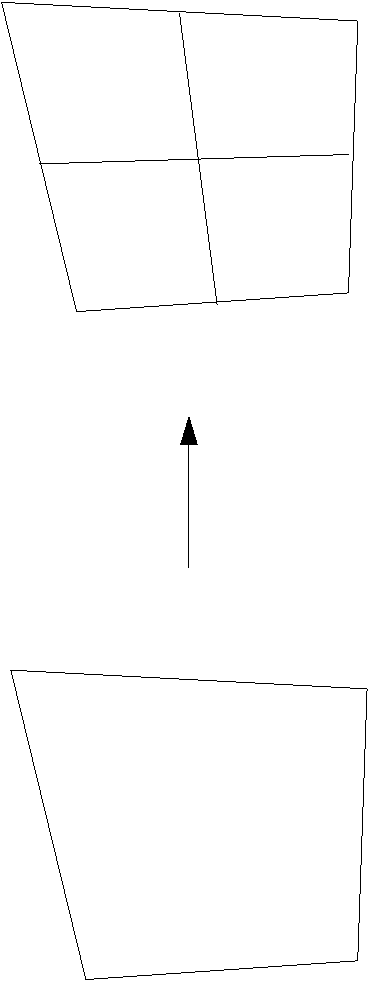
\includegraphics[angle=-90, width=.45\textwidth]{amr/quad_refinement} \\
    Triangle && Quadrilateral \\
    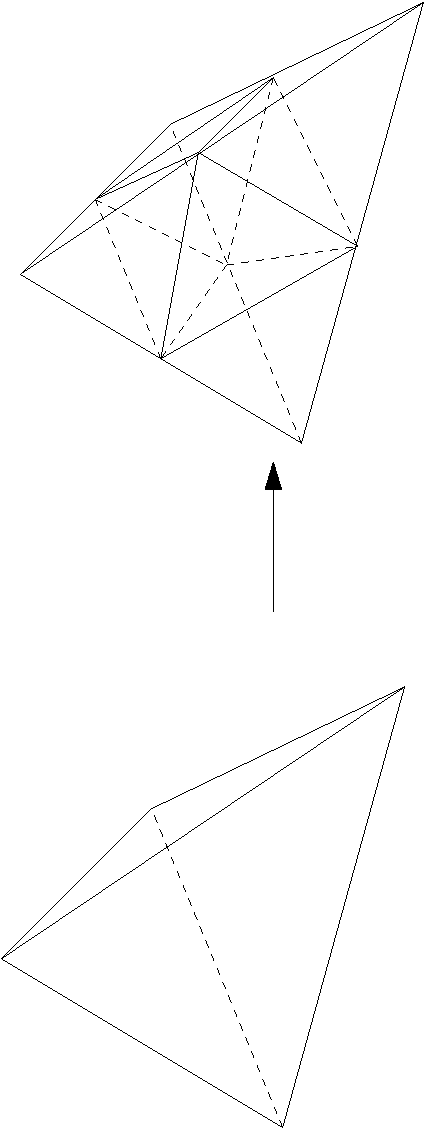
\includegraphics[angle=-90, width=.45\textwidth]{amr/tet_refinement} &&
    \includegraphics[angle=-90, width=.45\textwidth]{amr/prism_refinement}  \\
    Tetrahedron && Prism
  \end{tabular}
\end{frame}


%%%%%%%%%%%%%%%%%%%%%%%%%%%%%%%%%%%%%%%%%%%%%%%%%%%%%%%%%%%%%%%%%%%%%%%%%%%%%%%
\begin{frame}{Flux-Jump Error Indicator}
\begin{itemize}
\item The flux-jump error indicator is derived starting from the element
  integrals
  % Reference the previously used equation with the same number
    \begin{equation}
      \eqneltint\tag{\ref{eqn:element_integrals}}
    \end{equation}

  \item Applying the divergence theorem ``in reverse'' obtains
    \begin{eqnarray}
      \sum_{e=1}^{N_e} \int_{\Omega_e}
      \left( -\Delta u^h  + (\bv{b} \cdot \nabla u^h) + cu^h
      -f \right) v^h \;  dx + \\
      \nonumber
      \sum_{\partial \Omega_e \not \subset  \partial \Omega}
      \int_{\partial \Omega_e} \left\llbracket \frac{\partial u^h}{\partial n} \right\rrbracket v^h \; dx=0
    \end{eqnarray}
\end{itemize}
\end{frame}


%%%%%%%%%%%%%%%%%%%%%%%%%%%%%%%%%%%%%%%%%%%%%%%%%%%%%%%%%%%%%%%%%%%%%%%%%%%%%%%
\begin{frame}{Flux-Jump Error Indicator (cont.)}
  \begin{itemize}
  \item Defining the cell residual
    \begin{equation}
      r(u^h) = -\Delta u^h  + (\bv{b} \cdot \nabla u^h) + cu^h -f
    \end{equation}
    we have
    \begin{eqnarray}
      \label{eqn:residuals}
      \sum_{e=1}^{N_e} \int_{\Omega_e}
      r(u^h) v^h \;  dx +
      \sum_{\partial \Omega_e \not \subset  \partial \Omega}
      \int_{\partial \Omega_e} \left\llbracket \frac{\partial u^h}{\partial n} \right\rrbracket v^h \; dx=0
    \end{eqnarray}

  \item Clearly, the exact solution $u$ satisfies~\eqref{eqn:residuals} identically.

  \item Computing $r(u^h)$ requires
    knowledge of the differential operator (i.e.\ knowledge of the ``physics'').

  \item The second sum leads to a \emph{physics-independent} method for estimating the
    error in the approximate solution $u^h$.

  \end{itemize}
\end{frame}



%%%%%%%%%%%%%%%%%%%%%%%%%%%%%%%%%%%%%%%%%%%%%%%%%%%%%%%%%%%%%%%%%%%%%%%%%%%%%%%
\begin{frame}{1D Example}
  \begin{columns}
    \column{.65\textwidth}
    \begin{itemize}
    \item Consider the function
      \begin{equation}
        \nonumber
        u = \frac{1-\exp(10x)}{1-\exp(10)}
      \end{equation}
      which is a solution of the classic 1D advection-diffusion boundary layer equation.
\item We assume here that the finite element solution is the linear
  interpolant of $u$, and compute the error indicator for a sequence of
  uniformly refined grids.
\end{itemize}

      \column{.35\textwidth}
  \begin{center}
    \includegraphics[viewport=50 50 700 600,width=.9\textwidth]{amr/bl}
  \end{center}
  \end{columns}
\end{frame}



%%%%%%%%%%%%%%%%%%%%%%%%%%%%%%%%%%%%%%%%%%%%%%%%%%%%%%%%%%%%%%%%%%%%%%%%%%%%%%%
\begin{frame}%{1D Example (cont.)}
  \only<1>
  {
    \begin{tabular}{cc} \\
      \includegraphics[angle=-90,width=.42\textwidth]{amr/u_bl_5elems}&
      \includegraphics[angle=-90,width=.42\textwidth]{amr/up_bl_5elems} \\
      \includegraphics[angle=-90,width=.42\textwidth]{amr/eta_bl_5elems}&
      $\begin{array}{c}
        \text{4 elements} \\
        ||e||_{L_2} = 0.09
      \end{array}$\\
    \end{tabular}
  }
  \only<2>
  {
    \begin{tabular}{cc} \\
      \includegraphics[angle=-90,width=.42\textwidth]{amr/u_bl_9elems}&
      \includegraphics[angle=-90,width=.42\textwidth]{amr/up_bl_9elems} \\
      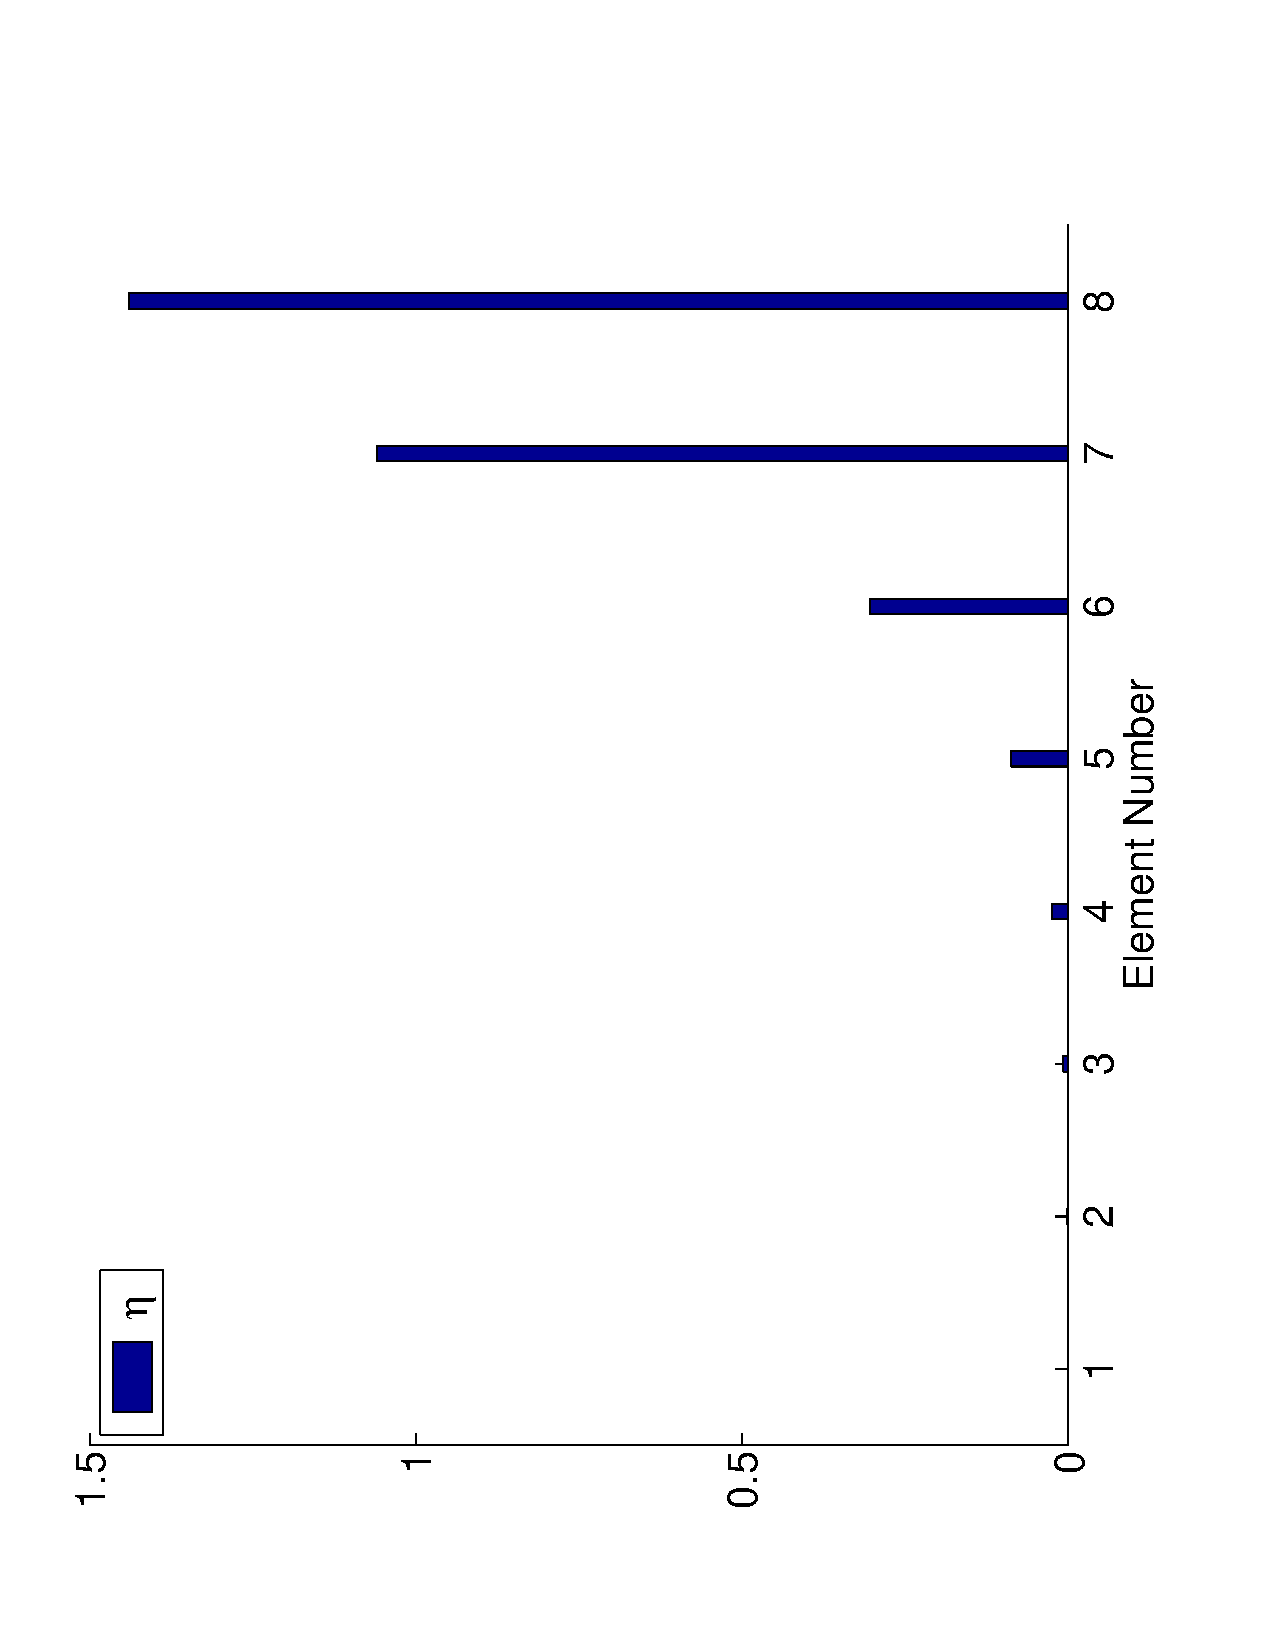
\includegraphics[angle=-90,width=.42\textwidth]{amr/eta_bl_9elems}&
      $\begin{array}{c}
        \text{8 elements} \\
        ||e||_{L_2} = 0.027
      \end{array}$\\
    \end{tabular}
  }
  \only<3>
  {
    \begin{tabular}{cc} \\
      \includegraphics[angle=-90,width=.42\textwidth]{amr/u_bl_17elems}&
      \includegraphics[angle=-90,width=.42\textwidth]{amr/up_bl_17elems} \\
      \includegraphics[angle=-90,width=.42\textwidth]{amr/eta_bl_17elems}&
      $\begin{array}{c}
        \text{16 elements} \\
        ||e||_{L_2} = 0.0071
      \end{array}$\\
    \end{tabular}
  }
\end{frame}



%%%%%%%%%%%%%%%%%%%%%%%%%%%%%%%%%%%%%%%%%%%%%%%%%%%%%%%%%%%%%%%%%%%%%%%%%%%%%%%
\begin{frame}[fragile]{A Simple Refinement Strategy}

  \begin{itemize}
    \item A simple adaptive refinement strategy with \texttt{r\_max} refinement steps
      for this 1D example problem is:
  \end{itemize}

%%   \begin{enumerate}
%%   \item Determine an initial grid (e.g. two elements)
%%   \item Compute the FE solution (linear interpolant)
%%   \item Estimate the error in the FE solution using the flux-jump indicator
%%   \item Refine (by splitting) the elements whose error is in the top 10\%
%%   \item Return to step 2.
%%   \end{enumerate}

\small
\begin{semiverbatim}
r=0;
while (r < r_max)
  Compute the FE solution (linear interpolant)
  Estimate the error (using flux-jump indicator)
  Refine the elements with error in top 10\%
  Increment r
end
\end{semiverbatim}
\end{frame}


%%%%%%%%%%%%%%%%%%%%%%%%%%%%%%%%%%%%%%%%%%%%%%%%%%%%%%%%%%%%%%%%%%%%%%%%%%%%%%%
\begin{frame}
  \only<1> {  \includegraphics[width=.7\textwidth,angle=-90]{amr/adaptive_u_bl_2elems} }
  \only<2> {  \includegraphics[width=.7\textwidth,angle=-90]{amr/adaptive_u_bl_3elems} }
  \only<3> {  \includegraphics[width=.7\textwidth,angle=-90]{amr/adaptive_u_bl_4elems} }
  \only<4> {  \includegraphics[width=.7\textwidth,angle=-90]{amr/adaptive_u_bl_5elems} }
  \only<5> {  \includegraphics[width=.7\textwidth,angle=-90]{amr/adaptive_u_bl_6elems} }
  \only<6> {  \includegraphics[width=.7\textwidth,angle=-90]{amr/adaptive_u_bl_7elems} }
  \only<7> {  \includegraphics[width=.7\textwidth,angle=-90]{amr/adaptive_u_bl_8elems} }
  \only<8> {  \includegraphics[width=.7\textwidth,angle=-90]{amr/adaptive_u_bl_9elems} }
  \only<9> {  \includegraphics[width=.7\textwidth,angle=-90]{amr/adaptive_u_bl_10elems} }
  \only<10> {  \includegraphics[width=.7\textwidth,angle=-90]{amr/adaptive_u_bl_11elems} }
  \only<11> {  \includegraphics[width=.7\textwidth,angle=-90]{amr/adaptive_u_bl_13elems} }
\end{frame}



%%%%%%%%%%%%%%%%%%%%%%%%%%%%%%%%%%%%%%%%%%%%%%%%%%%%%%%%%%%%%%%%%%%%%%%%%%%%%%%
\begin{frame}{A Simple Refinement Strategy (cont.)}
  \includegraphics[height=.9\textheight]{amr/error_plot}
\end{frame}


%%%%%%%%%%%%%%%%%%%%%%%%%%%%%%%%%%%%%%%%%%%%%%%%%%%%%%%%%%%%%%%%%%%%%%%%%%%%%%%
\begin{frame}
\frametitle{Goal-oriented Adaptivity}

\begin{columns}

\column{0.5\textwidth}
Refine to reduce solution error {\emph{when it influences QoI error}}:

\begin{center}
\includegraphics[width=1.0\textwidth]{qoi_may_29_2009_convergence_cropped}
\end{center}

\column{0.45\textwidth}

\begin{center}
\includegraphics[height=0.5\textwidth]{QoI_October_20_2011_kelly_mesh}
\includegraphics[height=0.5\textwidth]{QoI_May_29_2009_arpp_mesh+adjoint}
\end{center}

\begin{itemize}
\item Global error indicator targets layer alone; QoI temporarily plateaus
\item Rapid convergence from adjoint-based refinement
\end{itemize}

\end{columns}

\end{frame}


\begin{frame}
\frametitle{Adaptivity: Error Estimators, Error Indicators}
\begin{columns}
\column{.7\textwidth}
\begin{block}{Error decompositions}
        Subterms on each element $K$:
        \begin{itemize}
                \item $\norm{u-u_h}_\mathcal{H}^2 = 
                        \sum_K \norm{u-u_h}_\mathcal{H(K)}^2 \leq 
                        \sum_K \abs{\eta_K}^2$
                \item $\Qoi(u) - \Qoi(u_h) \approx \sum_K \eta_K$
                \item $\abs{\Qoi(u) - \Qoi(u_h)} \leq \sum_K \abs{\eta_K}$
        \end{itemize}
\end{block}
\begin{block}{Refinement heuristics}
        \begin{itemize}
        \item Refinement/coarsening of elements with:
        \begin{itemize}
                \item Worst/best fraction sorted by error
                \item Error over/under fraction of tolerance
                \item Error over/under target mesh size average
        \end{itemize}
        \item $h$-vs-$p$ refinement:
        \begin{itemize}
                \item {\textit{a priori}} singularity identification
                \item Behavior vs. cost when $h$ vs. $p$ coarsening?
        \end{itemize}
        \end{itemize}
\end{block}

\column{.3\textwidth}
\center
\includegraphics[width=.6\textwidth]{qoi_primal_error}

\center
\includegraphics[width=.6\textwidth]{qoi_weighted_error}
\end{columns}
\end{frame}



\begin{frame}
\frametitle{Adjoint-based Error Indicators, Sensitivities}

\vspace{-5mm}

\begin{eqnarray*}
\Qoi(\primalsolh) - \Qoi(\primalsol) & = & \Res(\primalsolh, \adjointsol - \adjointsolh) + H.O.T. \\
\qoi' & = & \Qoi_\params(\primalsol; \params) - 
        \Res_\params(\primalsol, \adjointsol - \Liftfunc(\primalsol; \params); \params)
\end{eqnarray*}

\begin{block}{Adjoint Refinement}
\begin{equation*}
\Res(\primalsolh, \adjointsol - \adjointsolh) \approx \sum_\elem 
\Res^\elem(\primalsolh, \adjointsolH - \adjointsolh)
\end{equation*}
\end{block}

\begin{block}{Adjoint Residual}
\vspace{-4mm}
\begin{equation*}
\abs{\Res(\primalsolh, \adjointsol - \adjointsolh)} \leq
\sum_\elem \norm{\Res^\elem_\unknown}_{B(\Unknowns^\elem,
\Testfuncs^{\elem *})}
\norm{\primalsol - \primalsolh}_{\Unknowns^\elem}
\norm{\adjointsol - \adjointsolh}_{\Testfuncs^\elem}
\end{equation*}
\end{block}

\begin{block}{Generalized Adjoint Residual}
\vspace{-4mm}
\begin{align*}
\abs{\Res(\primalsolh, \adjointsol - \adjointsolh)}
\leq \sum_\elem \norm{\adjointsol_i-\adjointsolh_i}_i \; M_{ij} \; \norm{\primalsol_j-\primalsolh_j
}_j \nonumber
\end{align*}
\end{block}

\end{frame}



%% \end{document}

%% Local Variables:
%% mode: latex
%% End:
